\section{zkSharding Architecture}
\label{sec:architecture}

\todoisinline{The figure 2 is too big and complex

	\handan{I removed it but it can be good to have a figure giving
		the
		overall design. If we have something like this we can put
		it.}}
%\begin{figure}
%	\centering
%	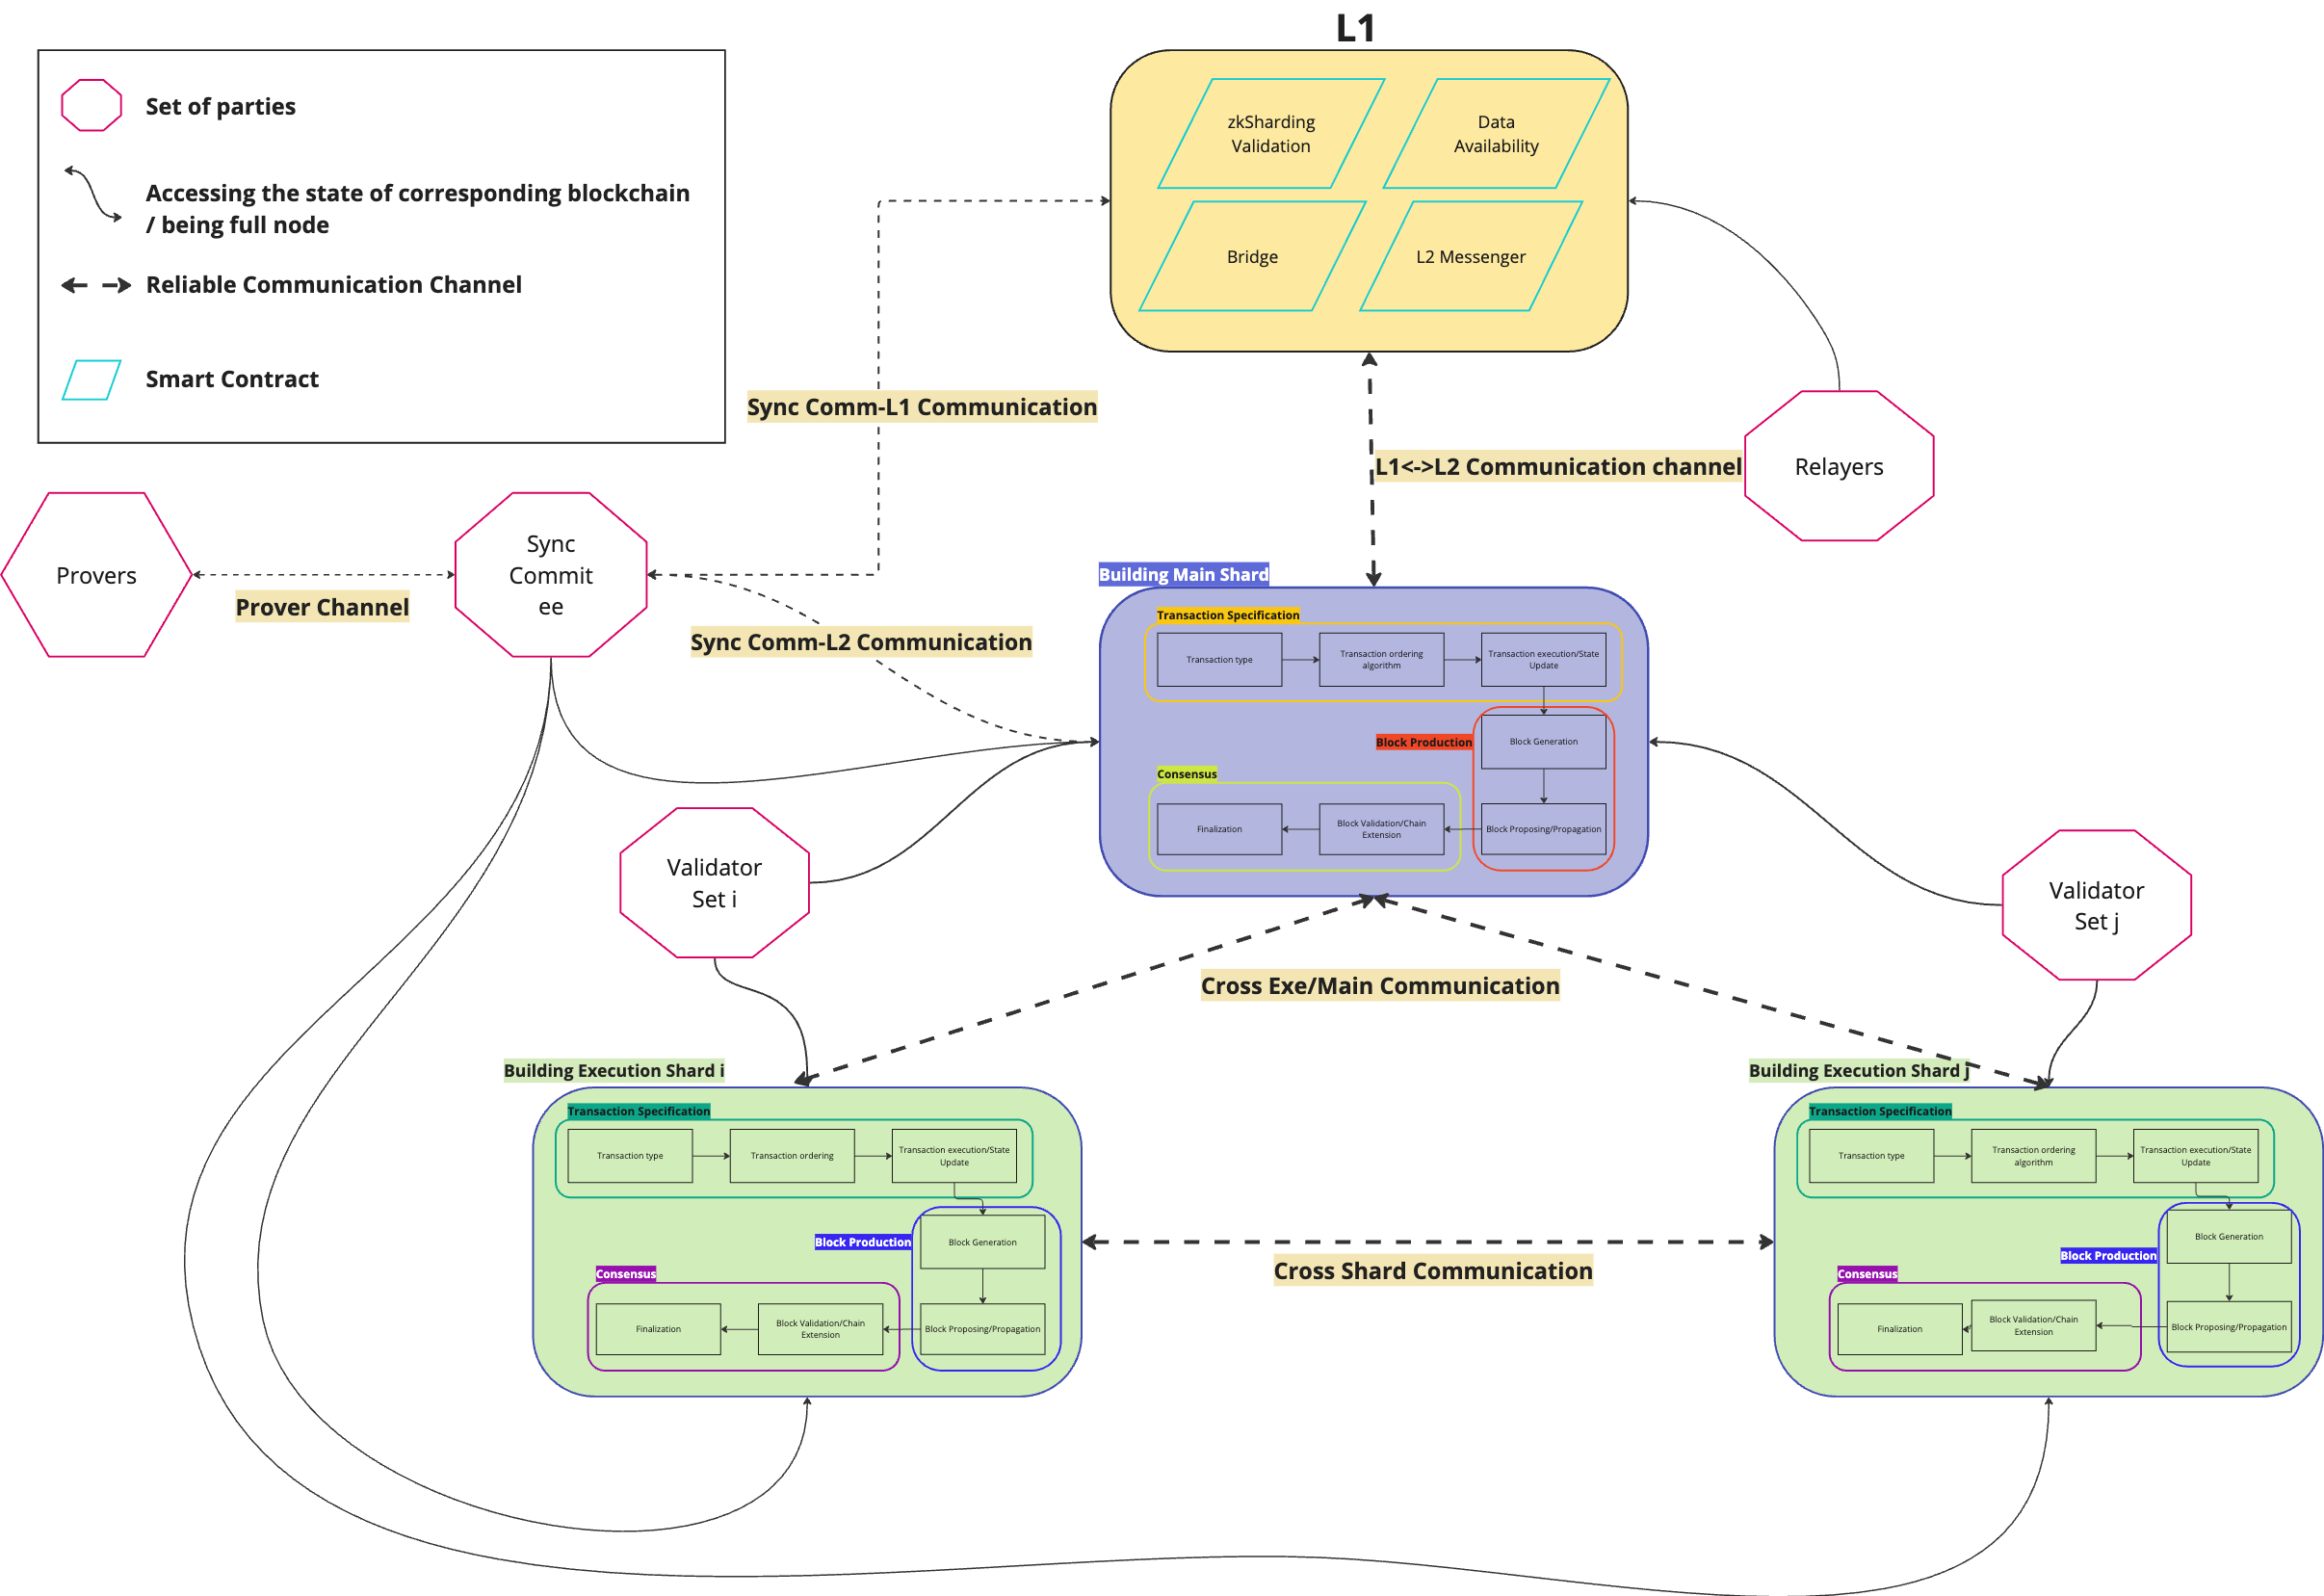
\includegraphics[width=1\linewidth]{figures/components}
%	\caption{zkSharding Components}
%	\label{fig:components}
%\end{figure}
\short{
	As previously discussed, zkSharding operates across three
	interconnected components. Each component serves a distinct
	function, yet they
	work together to ensure  scalability and security. In this
	section, we explore how they are
	linked and describe the architecture that enables state
	synchronization. We
	also introduce the key actors who play critical roles in the
	system.
}{
	As previously discussed, zkSharding operates across three
	interconnected components: L1, the main shard, and multiple
	execution shards.
	Each component serves a distinct function, yet they work together
	to ensure
	scalability, security, and seamless operation of the system. In
	this section, we explore how these layers are
	linked, describing the architecture that enables efficient data
	flow and
	state synchronization. We also introduce the key actors, such as
	validators, provers, and the sync committee, who play critical
	roles in
	maintaining the integrity and security of zkSharding by
	facilitating
	communication and consensus between the layers.
}

\subsection{Actors}

The core participants in zkSharding’s architecture are
\emph{\textbf{validators}}, who play vital roles across different layers.
Each validator $\val_i$ joins the network by staking a certain amount of
funds which incentivizes to maintain the security of the system.
Validators can
operate in multiple roles:

Validators are responsible from building and maintaining the main shard
and execution shards. When operating the main shard, they participate in
running the \emph{global} consensus algorithm which helps to the
synchronization of states across all execution shards.	In the execution
shards, validators are responsible for executing shard-specific
transactions and maintaining its local consensus. Beyond this, validators
can be the part of the synchronization committee $\syncSet$. The members
of $\syncSet$ are responsible for interfacing zkSharding with L1. They
manage tasks like submitting data, proofs, and transactions to the L1
contracts outlined in Section \ref{sec:l1}. The committee is re-elected
each epoch based on protocol parameters, and only validators opting for
this role participate. To maintain clear role separation, a validator
cannot simultaneously serve on both the main shard and the $\syncSet$
committee.

%\begin{itemize}
%	\item \textbf{Main Shard Validators:} These validators are
%	      responsible for building and maintaining the Main Shard. They participate
%	      in running the \emph{global} consensus algorithm that ensures the
%	      synchronization of states across execution shards.
%
%	\item \textbf{Execution Shard Validators:}
%	      \short{
%		      Each execution shard $\shard_i$ has its own set of
%		      validators, $\valset_i$, drawn from the main shard validator set,
%		      $\valset$. These validators are responsible for block creation, executing
%		      transactions, and maintaining \emph{local} consensus in their shard,
%		      $\shard_i$. 
%	      }{
%		      Each execution shard $\shard_i$ has its own subset of
%		      validators, drawn from the main shard validator set $\valset$. We denote
%		      the set of validators specific to an execution shard as $\valset_i$. These
%		      validators are tasked with building blocks, executing transactions, and
%		      running the local consensus mechanism within their assigned execution
%		      shard $\shard_i$. 
%	      }
%
%	\item \textbf{Synchronization Committee:}
%	      \short{
%		      The committee $\syncSet$ is a  group of validators
%		      responsible for interfacing zkSharding with L1. They manage tasks like
%		      submitting data, proofs, and transactions to the L1 contracts outlined in
%		      Section \ref{sec:l1}. The committee is re-elected each epoch based on
%		      protocol parameters, and only validators opting for this role participate.
%		      To maintain clear role separation, a validator cannot simultaneously serve
%		      on both the main shard and the $\syncSet$ committee.
%	      }{
%		      This committee $\syncSet$ is a subset of validators
%		      responsible for interfacing zkSharding with L1. They handle the critical
%		      task of submitting data, proofs, and transactions to the L1 contracts
%		      discussed in Section \ref{sec:l1}. The committee is dynamically elected at
%		      the beginning of each epoch, based on protocol-defined parameters, and
%		      consists of validators who opt into this additional responsibility.
%		      Importantly, to maintain role separation, an account cannot act as both a
%		      main shard validator and a member of $\syncSet$ simultaneously. This
%		      ensures that funds staked by committee members are subject to slashing
%		      only for infractions related to their specific role.
%	      }
%	      By distributing responsibilities across a dynamically elected
%	      group of validators, zkSharding prevents centralization of power, reducing
%	      the risk of collusion or censorship. This ensures the system remains
%	      robust, even if some committee members act maliciously or fail in their
%	      duties.
%\end{itemize}

\short{
	In addition to validators, zkSharding has a role
	\emph{\textbf{prover}}. Each prover $\prover$ is part of a
	dedicated
	proving network and is responsible for executing zkSharding’s
	proving
	algorithm (see Section \ref{sec:zkp}).
}{
	In addition to validators, zkSharding has a role
	\emph{\textbf{prover}}. Each prover $\prover$ is part of a
	dedicated
	proving network and is responsible for executing zkSharding’s
	proving
	algorithm (see Section \ref{sec:zkp}). They generate cryptographic
	proofs
	that verify the correctness of transactions and state transitions,
	which
	are then submitted to validators in $\syncSet$ for further
	processing and
	eventual inclusion on L1.
}
\handan{Should we tell anything about prover fees? Do they get their fee
	from the main shard? Or are they independent actors receiving
	their fee
	from the sync commitee?}

\short{
	Furthermore, there is the role of \emph{\textbf{relayers}}, who
	ensure the reliable transmission of contract calls from Ethereum
	to
	zkSharding.
}{Furthermore, there is the role of \emph{\textbf{relayers}}, who ensure
	the reliable transmission of contract calls from Ethereum to
	zkSharding.
	Relayers facilitate actions such as deposit contract calls,
	guaranteeing
	that messages are reliably delivered to the appropriate components
	within
	zkSharding. This role is integral to zkSharding’s bridge design.
}

\subsection{Components}

In this section, we describe the structure and functionality of the main
shard and execution shards.
\subsubsection{Main Shard:}
Main shard functions as a specialized blockchain that manages operational
transactions crucial to the integrity of zkSharding. The key operational
transactions are as follows:

\begin{itemize}
	\item \textbf{Validator Rotation Algorithm:}
	      Main shard runs a dedicated algorithm, referred to
	      as the
	      \emph{Validator Rotation Algorithm} \cite{rotation},
	      which randomly
	      assigns validators to execution shards. It is
	      optimized to ensure that
	      each execution shard has a sufficient number of
	      honest validators to
	      guarantee safety and reliability.
	      The algorithm divides validators into two groups:
	      large-stake
	      validators (above a set threshold) and smaller-stake
	      validators. It
	      ensures that each execution shard has a balanced
	      representation,
	      prioritizing larger-stake validators for their
	      trustworthiness.
	      Additionally, it enforces a minimum number of
	      validators per shard to
	      promote decentralization and reduce the risk of
	      centralization. This
	      approach maintains fairness, ensuring even
	      distribution of trustworthy
	      validators while guaranteeing that every shard has
	      sufficient validators
	      to operate securely.

	      \begin{enumerate}
		      \item The proportion of large stake validators in
		            each execution shard must be at least
		            $\ratioLexe$.
		      \item The variance in the proportion of large
		            stake validators across all execution shards
		            should not exceed
		            $\distance$.
		      \item Each execution shard must have at least
		            $\lmin$ validators.
	      \end{enumerate}

	      Notably, a validator with a large stake can be assigned to
	      multiple execution shards if necessary.

	      The purpose of the first constraint is to maintain a
	      minimum level of participation from large stake validators,
	      as they are
	      considered more trustworthy. The second constraint ensures
	      that this trust
	      is evenly distributed across multiple shards, avoiding
	      scenarios where a
	      few shards dominate the network. The third constraint
	      prevents
	      centralization by enforcing a minimum validator count for
	      each shard,
	      promoting a more decentralized architecture. More details on
	      the validator
	      allocation algorithm can be found in \cite{}.

	\item \textbf{Randomness Generation:}
	      To support unpredictability outcome of some protocols in
	      zkSharding, the main shard incorporates a
	      randomness generation mechanism.

	\item \textbf{Staking and Slashing:} Validators lock up a certain
	      amount of \emph{stake} when joining the network, which acts
	      as collateral
	      against dishonest behavior. The staking mechanism manages
	      this process,
	      while the slashing protocol penalizes validators for
	      malicious actions.

	\item \textbf{Bridge-Related Operations:}
	      \short{
		      The main shard is responsible for managing
		      operations
		      related to bridging assets and data between
		      zkSharding and Ethereum.
	      }{
		      The main shard is responsible for managing
		      operations
		      related to bridging assets and data between
		      zkSharding and Ethereum. This
		      includes coordinating contract calls, handling token
		      transfers, and
		      ensuring reliable messaging between zkSharding and
		      external blockchain
		      networks.
	      }

	\item \textbf{Finalizing Execution Shard Blocks:} Once an
	      execution shard completes a block, its header is submitted
	      to the main
	      shard, which verifies and finalizes the block header by
	      including it in the
	      global consensus (see Section \ref{sec:globalconsensus})
\end{itemize}

The main shard functions similarly to a referee in a
game.\todois{Comparison creates a feeling of centraliation around main
	shard \handan{How about now?}} Its role is to verify the block
headers from execution shards to validate that each shard adheres to
network rules.	\todois{Technically, it doesn't
	validate the most part of the ES block
	\handan{Done}}
This setup ensures that all execution shards maintain a synchronized view.
It is achieved by the global consensus provided by the main shard.
%Instead, they can
%simply check whether the respective block has been finalized by the main
%shard. This ensures that all execution shards share the same, consistent
%view of the network state.

\short{
	The global consensus in the main shard coordinates and
	synchronizes the states of all execution shards. It provides a
	consistent and
	unified system state. This internal process is distinct from L1
	consensus,
	which validates and finalizes the state of both the main shard and
	execution shards by verifying state validity proofs. While L1
	guarantees
	the validity of zkSharding's state, it is not involved in the
	internal
	synchronization or consensus mechanisms of zkSharding, which focus
	on
	managing shard execution and coordination,
}{
	In more detail, the purpose of global consensus in the main shard
	is to
	synchronize the states across all execution shards. It provides
	consistency
	and agreement on the overall state of the system. Importantly,
	this global
	consensus mechanism is an \emph{internal, operational} process
	within
	zkSharding. It is separate from the L1 consensus.
	The L1 consensus mechanism ultimately finalizes the states of both
	the main shard and the execution shards by verifying the proofs
	that
	zkSharding submits. In this way, L1 ensures that the states of all
	shards
	are valid and finalized, but it is not directly involved in the
	internal
	consensus mechanisms of zkSharding itself,  because the internal
	consensus
	mechanism is related to execution and coordination between
	execution
	shards.
}
In a nutshell, L1 consensus offers an additional layer of protection
through Ethereum’s strong security guarantees. This design combines the
decentralized scalability benefits of sharding with Ethereum's proven
security.
To summarize the consensus layers shown in Figure \ref{fig:consensus}:
\begin{itemize}
	\item Execution shards	run local consensus with their \emph{own
		      validators} to maintain synchronization of their
	      state in the shard.
	\item The main shard runs global consensus with \emph{all
		      validators}, ensuring synchronization and
	      consistency of states across all
	      execution shards.
	\item L1 verifies and finalizes the states of both the main shard
	      and execution shards, ensuring overall zkSharding finality.
\end{itemize}

\begin{figure}
	\centering
	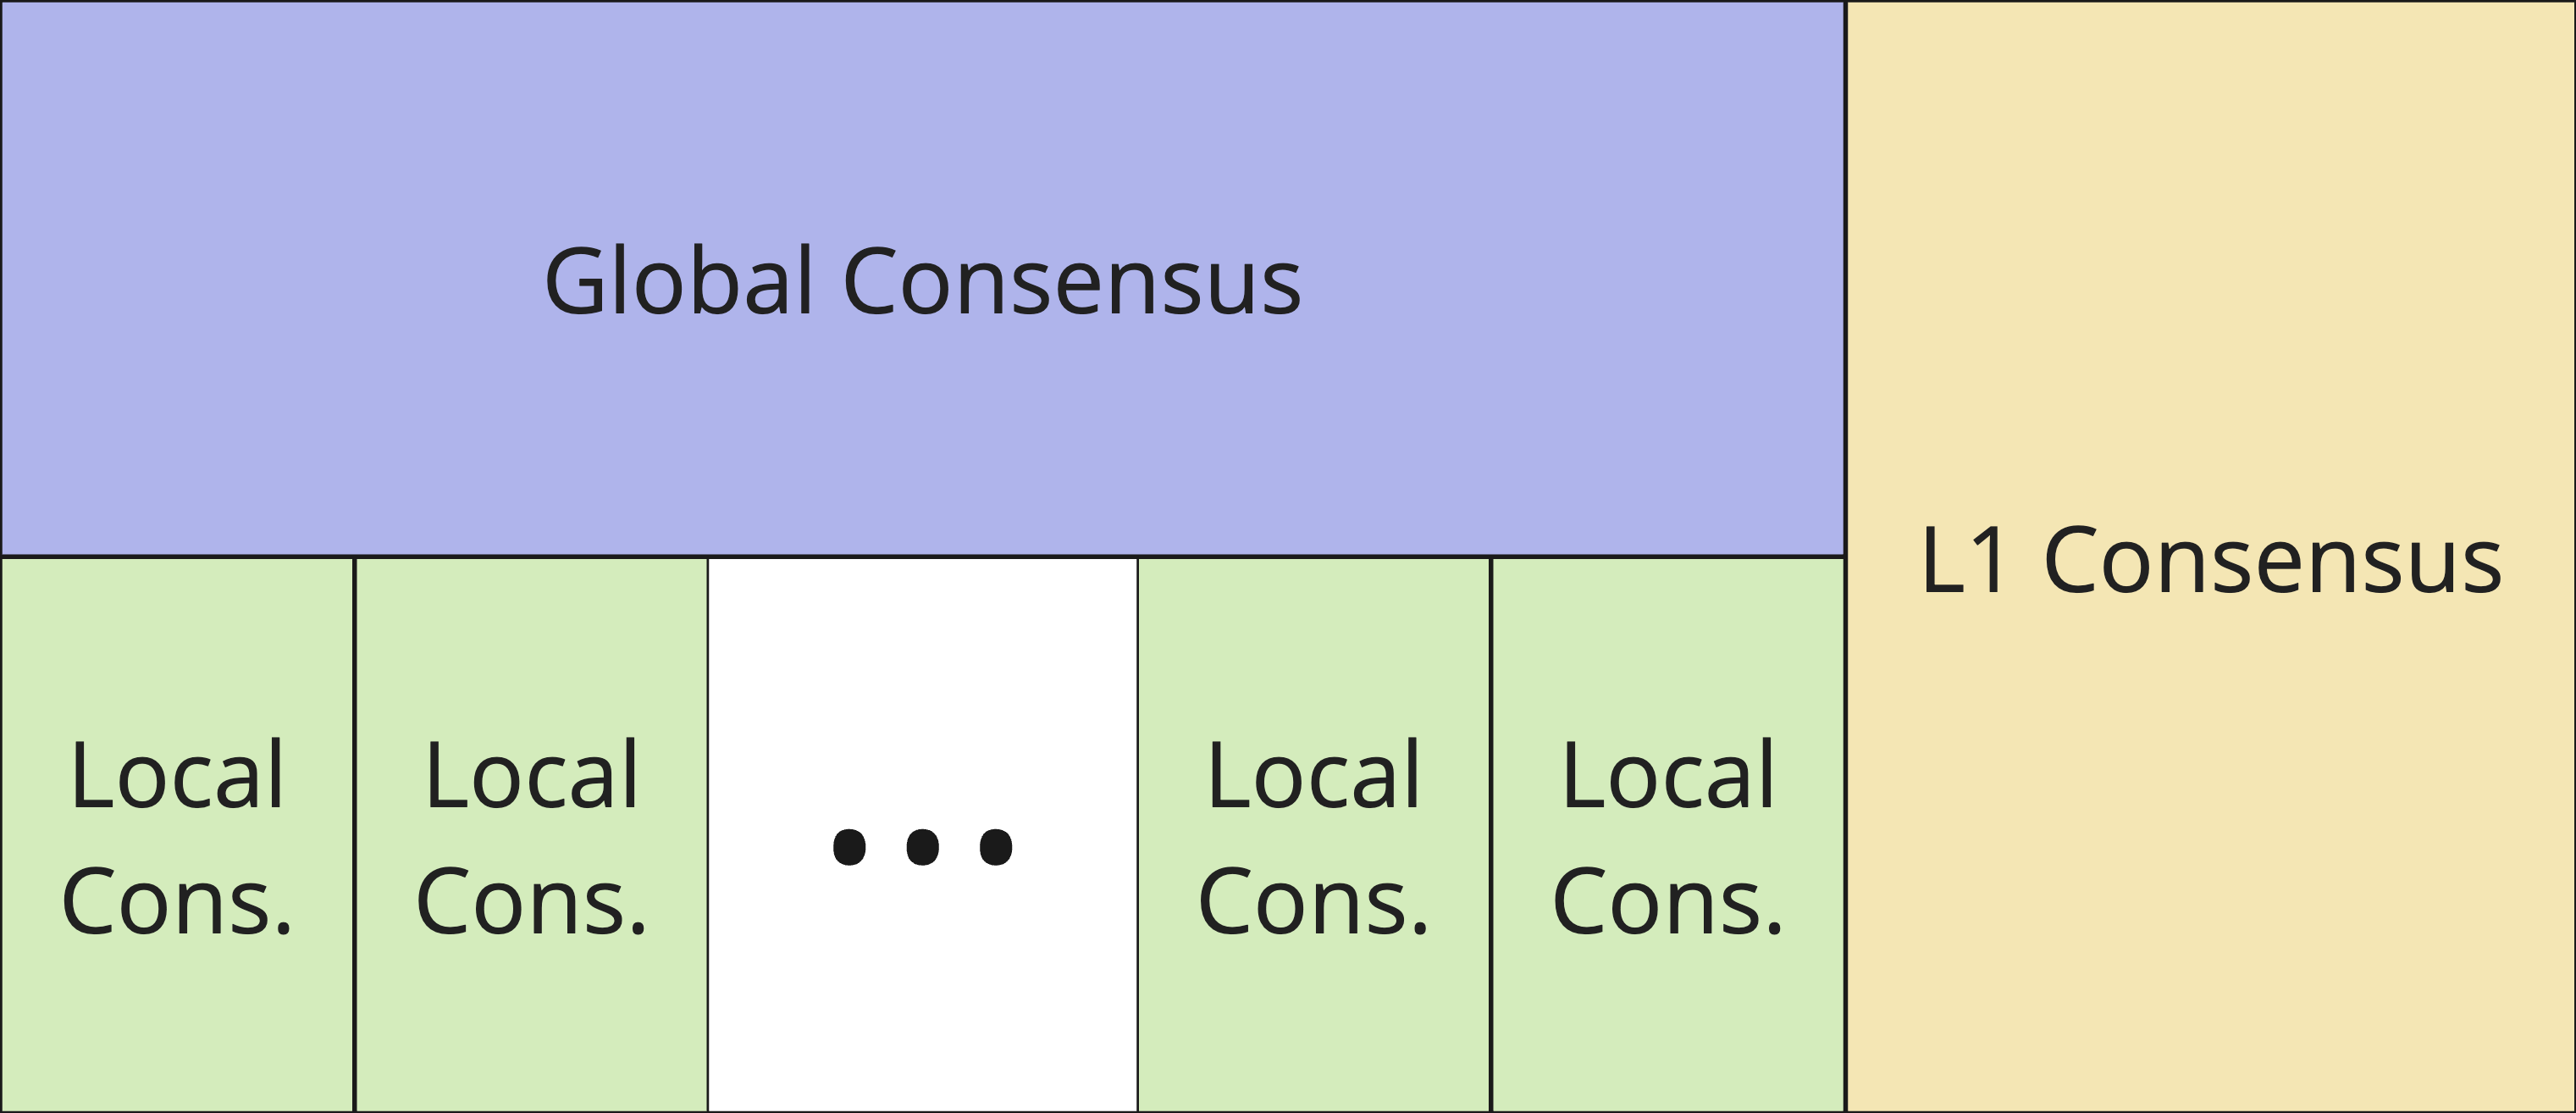
\includegraphics[width=0.5\linewidth]{figures/consensus}
	\caption{Consensus layers in zkSharding: Local consensus aligns
		execution shard states, global consensus by the main shard
		synchronizes
		them, and L1 consensus on Ethereum finalizes the state of
		both main and
		execution shards for overall system security.}
	\label{fig:consensus}
\end{figure}

\subsubsection{Execution Shard}
\label{sec:executionshards}
\todoisinline{The section is not about execution shards but about
	cross-shard comms. We need to include async-related stuff here
	\handan{I added information about acoounts, mempool, message
		delivery, async call, enshrined token design}}
In zkSharding, there are multiple execution shards, each managing its own
set of accounts. An account is the fundamental data unit in each shard and
includes the address, balance, storage root, and a hash of the contract’s
source code. Notably, all accounts in zkSharding are represented by smart
contracts. By structuring all accounts as smart contracts, zkSharding
centralizes operational logic across the system. It simplifies message
handling and state updates.

Each execution shard operates a dedicated mempool that temporarily stores
external messages sent by users, dApps, or other external sources. These
messages are queued in the mempool until the associated smart contract
processes them.
During contract execution, if a contract generates additional internal
messages to other contracts, these bypass the mempool and are instead
routed directly to their target contracts on either the same or another
shard. This direct routing avoids unnecessary queuing, creating a more
efficient and streamlined message processing flow across execution shards.

zkSharding deploys \emph{enshrined token design} \cite{tokenNil} in
execution shards which offers efficient approach to managing token
transaction across execution shards. With enshrined tokens, the core token
functions (like transfer, balance checking, and approvals) are directly
built into the core protocol of execution shards rather than being
implemented through smart contracts. This allows these operations to
benefit from protocol-level optimizations. In this way, the protocol
itself handles the complexity of moving tokens between execution shards.

Execution shards communicate through a
\emph{cross-shard communication protocol}. It guarantees that
messages between shards are
eventually executed. In this protocol, even execution shards which are not
message's
destination play a \textit{supporting} role by storing message-related
data, thereby helping to enforce eventual
execution on the destination shard. \todois{I understand what are you
	trying to explain, but this
	sentense may be more misleading fot the reader \handan{How is it
		now? If it is still misleading, I can remove it}}
To enable efficient communication between execution shards, zkSharding
allow smart contracts deployed on different execution shards to interact
without halting execution. The $\mathtt{asyncCall}$ function
\cite{asyncNil} is integral to this feature. It enables a contract on one
shard to call functions on contracts located on other shards directly,
without waiting for an immediate response. This mechanism produces a
message that is processed by the destination shard asynchronously,
allowing parallelism across shards and improving network scalability.

A unique data structure of our execution shards is the \textbf{ShardDAG}
\cite{sharddagEthResearch}. It is a structure that connects blocks from
different
execution shards as well as blocks from the main shard. This shared
structure imposes a global ordering of transactions that mitigates Maximum
Extractable Value (MEV) attacks \cite{mev1,mev2} especially for
cross-shard
transactions and guarantees ultimate cross-shard transaction processing.

\paragraph{ShardDAG:} It is inspired by DAG-based blockchains
\cite{dagSoK1,dagSoK2}, and operates as
follows:
When a validator generates a block $\block$ for execution shard
$\shard_i$, in addition to the transactions, it adds the following
elements to connect $\block$ to other blocks to form the DAG:
\begin{itemize}
	\item The hash of the latest block from the same shard $\shard_i$,
	      as in a typical blockchain.
	\item Hashes of blocks from other shards, following the ShardDAG
	      rules \cite{sharddag}, which act as acknowledgments that the
	      execution
	      shard has received data from those other shards.
	\item The hash of the latest main shard block to ensure that
	      cross-shard transactions are eventually processed and
	      recognized by the
	      entire network.
\end{itemize}

\begin{figure}
	\centering
	
\includegraphics[width=1\linewidth]{figures/shardDAGStrategy}
	\caption{ The ShardDAG rules enforce a strategy that ensures
		secure cross-shard transactions: (1) \textbf{Child
			Condition} enforces
		data availability by requiring broadcast to more than $F$
		shards; (2)
		\textbf{Parent Condition} guarantees receipt by
		integrating data from
		multiple shards; and (3) \textbf{Main-Parent  Condition}
		maintains order
		with the main shard. Together, these rules ensure secure
		processing and
		reduce exploitation risks.}
	\label{fig:strategy}
\end{figure}

The ShardDAG enforces rules that  are designed to maintain security, data
availability, and orderly processing of transactions. The key rules
include\todois{simplify to less strict definitions \handan{I was not sure
		how to be  less strict so I try to focus more on the
		purpose of the
		rules.}}:

\begin{itemize}
	\item \textbf{Child Condition:} An execution shard block is not
	      finalized until it has received acknowledgments from over
	      $F$ other
	      shards, where $F$ represents the system's tolerance for
	      potentially
	      adversarial shards. This condition helps ensure cross-shard
	      data is
	      sufficiently distributed, preventing single-shard control
	      over transaction
	      flow and supporting broad data availability.

	\item \textbf{Parent Condition:} An execution shard block must
	      have a subgraph that includes blocks from more than $F$
	      other shards
	      relative to its predecessor. This condition encourages
	      regular integration
	      of cross-shard data, reducing the risk of shards bypassing
	      or isolating
	      cross-shard transactions.

	\item \textbf{Main-Parent Condition  \handan{Check the name with
			      James. He refers it as consensus-parent
			      condition}:} A shard block should not
	      reference the same consensus block
	      for more than $X$ consecutive blocks, where $X$ depends on
	      the execution
	      shard's block time. This helps shards stay aligned with
	      updates from the
	      main shard. This promotes synchronization across the
	      network.
\end{itemize}

%LONGER VERSION
%\begin{itemize}
%	\item \textbf{Child Condition:} An execution shard block cannot be
%	      finalized until it is acknowledged by more than $F$ other shards. Here,
%	      $F$ represents the threshold derived from zkSharding’s adversarial
%	      assumptions, specifying the maximum number of potentially malicious shards
%	      that the system can tolerate. This rule ensures that cross-shard
%	      transaction data has been sufficiently broadcast and received across the
%	      network, reinforcing robust data distribution and preventing any single
%	      shard from stalling the transaction flow. By requiring acknowledgments
%	      from multiple shards, the system guarantees that cross-shard data
%	      availability is maintained.
%
%	\item \textbf{Parent Condition:} For an execution shard block to
%	      be considered valid, the graph difference between its subgraph and the
%	      subgraph of its previous block must contain blocks from more than $F$
%	      different shards.  This rule prevents any shard from bypassing the
%	      processing of cross-shard transactions or selectively isolating
%	      transactions, as it compels each shard to integrate data from multiple
%	      other shards, ensuring that cross-shard transactions are acknowledged and
%	      processed.
%
%	\item \textbf{Main-Parent Condition \handan{Check the name with
%			      James. He refers it as consensus-parent condition}:} A shard block is only
%	      considered valid if it has not created more than $X$  consecutive blocks
%	      referencing the same consensus block. The parameter $X$ depends on the
%	      block time of an execution shard. This rule ensures that shards stay
%	      synchronized with the main shard’s state and prevents any shard from
%	      endlessly producing blocks that do not account for new information from
%	      the main shard. This condition enforces consistent synchronization across
%	      the network.
%\end{itemize}

\short{
	See Figure \ref{fig:strategy} for a detailed illustration of how
	these rules enforce constraints for succesfull and orderly
	execution of
	transactions.
}{
	By enforcing these ShardDAG rules, zkSharding guarantees that
	cross-shard transactions are processed securely, efficiently, and
	in an
	ordered manner. See Figure \ref{fig:strategy} for a detailed
	illustration
	of how these rules enforce constraints for successful
	execution.These
	rules also help to mitigate the risks of MEV exploitation and
	censorship,
	ensuring that malicious behavior cannot manipulate or delay
	transactions.
}

%
%\paragraph{Prover Network:}
% Provers in the zkSharding system are responsible for generating zkps for the entire batch of transactions and state updates. Each proof certifies that the state transitions within the batch are valid and that no malicious changes were made. Once generated, the proofs are sent back to the sync commitee.